82. а) $$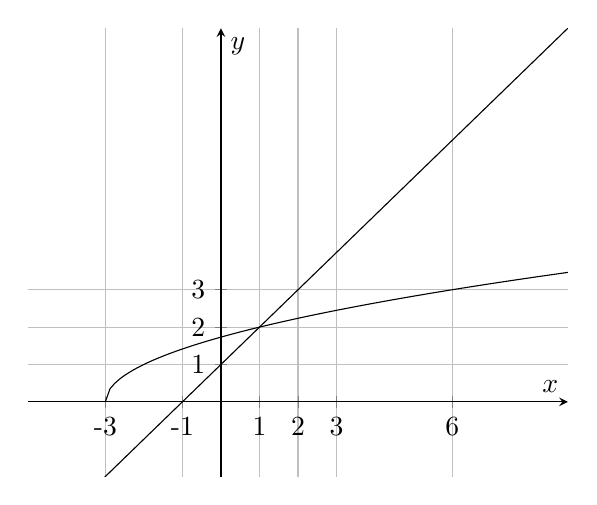
\begin{tikzpicture}[scale=1]
\begin{axis}[
    axis lines = middle,
    grid=major,
    legend pos={south west},
    xlabel = {$x$},
    %xlabel style={below right},
    ylabel = {$y$},
    ymin=-2,
    ymax=10,
    xmin=-5,
    xmax=9,
    xtick={-3,-1,1,2,3,6},
    xticklabels={-3,-1,1,2,3,6},
    ytick={3,2, 1},
    yticklabels={3,2, 1},
                  ]
	\addplot[domain=-3:9, samples=100, color=black] {sqrt(x+3)};
    \addplot[domain=-9:9, samples=100, color=black] {1+x};
        %\addplot[domain=2.01:6, samples=100, color=black] {2/(2-x)};
   % \addplot[domain=-3:3, samples=100, color=black] {-x};
     %\addlegendentry{$\text{Рис. 1}$};
\end{axis}
\end{tikzpicture}$$
По графику найдём ответ: $x\in[-3;1).$\\
б) Прямая $y=1+ax$ всегда проходит через точку $(0;1),$ и изменение параметра $a$ отвечает за её кручение вокруг этой точки. Если $a\leqslant0,$ то она пересечёт график $y=\sqrt{x+3}$ ровно один раз в левой полуплоскости. Если же $a>0,$ то она будет пересекать график два раза до тех пор, пока не пройдёт через точку $(-3;0),$ что произойдёт, когда $1-3a=0,\ a=\cfrac{1}{3}.$ При дальнейшем увеличении параметра $a$ прямая будет пересекать график только один раз в правой полуплоскости. Таким образом, $a\in(-\infty;0]\cup\left(\cfrac{1}{3};+\infty\right):$ 1 решение, $a\in\left(0;\cfrac{1}{3}\right]:$ 2 решения.\\
